
\section{Sample growth}

The samples were grown and initially characterised by Prof. Takeuchi's group in Sendai University, Japan in May 2009. \TODO{How were the Tc and compositions discovered? What technique was used for the growth?}. Stoichiometric \ac{BSCO} is overdoped. Adding La reduces the number of holes whereas adding Pb increases the number of holes. Also annealing in oxygen decreases the number of carriers depending on how much additional oxygen is absorbed. Table~\ref{Table:ExpH:SampleGrowthDetails} lists the nominal stoichiometries for the sample growth as well as the annealing conditions.
\begin{table}
    \begin{center}
           \caption{Growth details for the \ac{BSCO} samples. OD, OP and UD stand for over, optimally and under doped respectively.}
        {\small \begin{tabular}[htbp]{lllllllll}
\toprule
\multicolumn{6}{c}{Nominal composition} & & & \\
Bi  & Pb  & Sr  & La  & Cu  & O   & $T_c$   & Reg.  & Annealing conditions \\
\midrule
1.72    & 0.38  & 1.85  & 0.0   & 1.0   & 6+d   & $<$2  & OD    & \unit{400}{\celsius}, \unit{96}{\hour} in \unit{2.5}{\textrm{atm.}} O$_2$ \\
1.72    & 0.38  & 1.85  & 0.0   & 1.0   & 6+d   & 7     & OD    & \unit{750}{\celsius}, \unit{24}{\hour} in air \\
1.72    & 0.38  & 1.85  & 0.0   & 1.0   & 6+d   & 16    & OD    & \unit{550}{\celsius}, \unit{72}{\hour} in flowing N$_2$ \\
1.35    & 0.85  & 1.47  & 0.38  & 1.0   & 6+d   & 30    & OD    & As grown \\
1.35    & 0.85  & 1.47  & 0.38  & 1.0   & 6+d   & 32    & OP    & \unit{650}{\celsius}, \unit{72}{\hour} in flowing N$_2$ \\
1.2     & 0.90  & 1.30  & 0.55  & 1.0   & 6+d   & 30    & UD    & As grown \\
1.2     & 0.90  & 1.30  & 0.55  & 1.0   & 6+d   & 28    & UD    & \unit{650}{\celsius}, \unit{72}{\hour} in flowing N$_2$ \\
\bottomrule
        \label{Table:ExpH:SampleGrowthDetails}
        \end{tabular}}
    \end{center}
\end{table}

The samples are named according the convention,
\begin{quote}
\code{B<Tc>K<Region><Crystal No.><Sample No.>}
\end{quote}
so for example `B00KOD2A' refers to the sample `A' taken from the crystal `B00KOD2' --- the second overdoped crystal with a $T_c$ of $\unit{0}{K}$.

\section{Thickness measurements}

Thicknesses were determined for some of the samples using the \ac{FIB} or the optical microscope as described in the methods section. The results for various crystal samples used throughout this thesis are listed in table~\ref{Table:ExpH:Thicknesses}. \ac{FIB} results are given for areas as close to the two voltage contacts that were visible in the scans. As can be seen in the example scan shown in figure~\ref{Fig:ExpH:FIBExample}, there is some variation in the depth along the sample length. Measurements are therefore taken as close to the voltage legs as possible and whre appropriate suitable errors are estimated.
\begin{figure}[htbp]
	\begin{center}
		\includegraphics[scale=0.9]{CHapter-HallBSCO/FIgures/FIBExamples/FIBExamples}
		\caption{Top shows an image composited from several \ac{FIB} scans along the length of sample B00KOD1a, with bottom right showning a detail of the right voltage leg.  bottom left shows an oblique top down view of sample B30KOD3.}
		\label{Fig:ExpH:FIBExamples}
	\end{center}
\end{figure}

The two scans shown are of good quality, however for the purpose of estimating errors in the thickness some of the scans presented problems. Samples B26KOD1a, B28KUD3a, B30KOD2 and B30KUD3 were obscured with the grease applied as part of the pulsed field measurements. Other samples were not correctly earthed such as B28KUD3b which made the images dark, whilst samples B07KOD2 and B32KOP3 were very flakey under close scrutiny. A scan of B30KOD3 showed that it was partially split in the ab plane which may contribute to systematic error in thickness estimate. In all these cases, the esimate in the thickness error was adjusted accordingly to compensate. A more comprehensive set of \ac{FIB} scans, including images of the split in the layers can be found in Appendix~\ref{Appendix:FIBScans}.

The oblique view of B30KOD3 in figure~\ref{Fig:ExpH:FIBExample} shows a clear misalignment of the voltage legs to thr right of the image. This illustrates why it is necessary to take both positive and negative field sweeps in order to seperate the magnetoresistance from the Hall components.


\begin{table}
    \begin{center}
           \caption{Thickness measurements for the \ac{BSCO} samples as determined by \ac{FIB} and optical microscope measurements. A and B refer to each of the two contacts along one side. All measurements are in micrometres.}
        \begin{tabular}[htbp]{llll}
\toprule
Sample  & \ac{FIB} Contact A    & \ac{FIB} Contact B    & Optical   \\
\midrule
B00KOD1A	& $45\pm1$	& $50\pm5$	& N/A		\\
B00KOD1B	& $43\pm1.5$	& $45\pm1.5$	& $39\pm5$ 	\\
B07KOD1		& N/A		& N/A		& $29\pm10$	\\
B07KOD2		& $20\pm5$ 	& $30\pm1$ 	& N/A		\\
B16KOD1A	& $24\pm1$ 	& $24\pm1$ 	& N/A		\\
B16KOD2A	& N/A		& N/A		& $9\pm1$ 	\\
B16KOD3 	& $25\pm2$ 	& $24\pm2$ 	& N/A		\\
B30KUD2 	& $5 \pm1$ 	& $5 \pm1$ 	& N/A		\\
B30KOD1 	& N/A		& N/A		& $21\pm2$ 	\\
B30KOD2 	& $15\pm4$	& $15\pm4$	& $20\pm5$ 	\\
B30KOD3 	& $16.5\pm1.5$	& $19\pm1$	& N/A		\\
B32KOP1 	& $6.5\pm1.5$	& $6.5\pm1.5$	& N/A		\\
B32KOP2 	& N/A		& N/A		& $10\pm1$ 	\\
B32KOP3 	& $6\pm1$ 	& $6\pm1$ 	& N/A		\\
B32KOP4 	& $9\pm3$ 	& $9\pm3$ 	& N/A		\\
B30KUD1A	& N/A		& N/A		& $36\pm3$ 	\\
B30KUD1B	& N/A		& N/A		& $35\pm3$ 	\\
B30KUD3 	& $7\pm2$ 	& $7\pm2$ 	& N/A		\\
B28KUD2A	& N/A		& N/A		& $11\pm1$ 	\\
B28KUD3A	& $16\pm3$	& $16\pm3$	& N/A		\\
B28KUD3B	& $16\pm3$	& $16\pm3$	& N/A		\\
\bottomrule
        \label{Table:ExpH:Thicknesses}
        \end{tabular}
    \end{center}
\end{table}

\section{Field sweeps}

Figures~\ref{Fig:ExpH:HallIndividualOD}, \ref{Fig:ExpH:HallIndividualOP} and \ref{Fig:ExpH:HallIndividualUD} show the Hall coefficients extracted as described in the methods section for samples progressing from overdoped, optimally doped to underdoped respectively. Where appropriate, the data is compared to that from Ando \etal~\cite{Ando1999}. For the samples of $T_C >= \unit{28}{\kelvin}$ there are some data which did not reach sufficient field to obtain linear behaviour which are circled in the plots.

\begin{figure}[htbp]
	\begin{center}
		\includegraphics[scale=0.9]{Chapter-HallBSCO/Figures/HallIndividual/HallIndividualOD}
		\caption{$R_H$ for underdoped samples of \ac{BSCO}. Plots show results from, $\bullet$ Polo in June 2010, $\blacktriangle$ \ac{LNCMI} in June 2009, $\blacktriangledown$ \ac{LNCMI} in Feb 2010, $\blacksquare$ Nijmegen in May 2010. Symbols for comparable samples are marked on the plots.}
		\label{Fig:ExpH:HallIndividualOD}
	\end{center}
\end{figure}
\begin{figure}[htbp]
	\begin{center}
		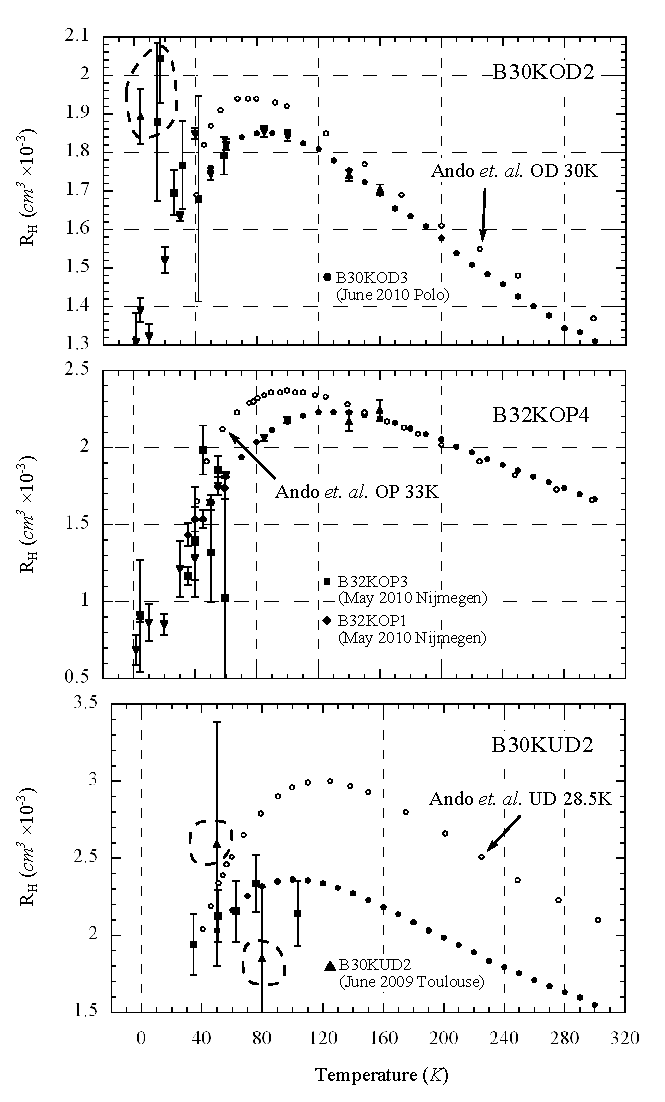
\includegraphics[scale=0.9]{Chapter-HallBSCO/Figures/HallIndividual/HallIndividualOP}
		\caption{$R_H$ for underdoped samples of \ac{BSCO}. Plots show results from, $\bullet$ Polo in June 2010, $\blacktriangle$ \ac{LNCMI} in June 2009, $\blacktriangledown$ \ac{LNCMI} in Feb 2010, $\blacksquare$ Nijmegen in May 2010. Symbols for comparable samples are marked on the plots. Dashed lines indicate points where the field was not sufficient to achieve linear behaviour.}
		\label{Fig:ExpH:HallIndividualOP}
	\end{center}
\end{figure}
\begin{figure}[htbp]
	\begin{center}
		\includegraphics[scale=0.9]{Chapter-HallBSCO/Figures/HallIndividual/HallIndividualUD}
		\caption{$R_H$ for underdoped samples of \ac{BSCO}. Plots show results from, $\bullet$ Polo in June 2010, $\blacktriangle$ \ac{LNCMI} in June 2009, $\blacktriangledown$ \ac{LNCMI} in Feb 2010, $\blacksquare$ Nijmegen in May 2010. Symbols for comparable samples are marked on the plots. Dashed lines indicate points where the field was not sufficient to achieve linear behaviour.}
		\label{Fig:ExpH:HallIndividualUD}
	\end{center}
\end{figure}
